% --------------------------------------------------------------
%                         Template DM
% --------------------------------------------------------------
\documentclass[11pt]{article} %draft = show box warnings
\usepackage[a4paper, total={6.5in,10.2in}]{geometry} % Flexible and complete interface to document dimensions
\renewcommand{\baselinestretch}{1.3} 

\usepackage[utf8]{inputenc} % accept different input encodings [utf8]
\usepackage[T1]{fontenc}    % Standard package for selecting font encodings
\usepackage{lmodern} % Good looking T1 font
% --------------------------------------------------------------
%                         Other Fonts
% --------------------------------------------------------------
%\usepackage{mathpazo} % Hermann Zapf's Palatino font
%\usepackage{kpfonts} % Kepler font
%\usepackage{mathptmx} % Times New Roman Like Font
%\usepackage{eulervm} %  aMS Euler (eulervm) math font.

% --------------------------------------------------------------
%                         Packages
% --------------------------------------------------------------
\usepackage[english]{babel} % Multilingual support
\usepackage{graphicx} % Enhanced support for graphics
\usepackage{float} % Improved interface for floating objects
\usepackage{amsmath,amsthm,amssymb} % american Mathematics Society facilities
\usepackage{hyperref}
\usepackage{listings}
\usepackage{color}
\usepackage{verbatim}
\usepackage[titletoc,toc,title]{appendix}
\usepackage{titlesec}
\usepackage{theoremref}
\usepackage{graphicx}
\usepackage{qtree}
\usepackage{tikz}
% --------------------------------------------------------------
%                       Task Env
% --------------------------------------------------------------
\newtheoremstyle{problemstyle}  % <name>
{3pt}                   % <space above>
{3pt}                   % <space below>
{\normalfont}           % <body font>
{}                      % <indent amount}
{\bfseries}             % <theorem head font>
{\normalfont\bfseries\hspace{0.2 cm}}  % <punctuation after theorem head>
{.5em}                  % <space after theorem head>
{}                      % <theorem head spec (can be left empty, meaning `normal')>
\theoremstyle{problemstyle}

% Change Language
\newtheorem{exercise}{Task}	% Englsih
%\newtheorem{exercise}{Exercice} 	% French
%\newtheorem{exercise}{Exercício}	% Pt-BR

% Change counter type
%\renewcommand{\theexercise}{\Roman{exercise}. } % Exercise I)
\renewcommand{\theexercise}{\arabic{exercise}.} % Exercise 1.
%\renewcommand{\theexercise}{\alph{exercise}.} % Exercise a.
%\renewcommand{\theexercise}{\alph{exercise}.} % Exercise a.

% --------------------------------------------------------------
%                       Comment Env
% --------------------------------------------------------------
\theoremstyle{problemstyle}
\newtheorem{commental}{Comment}
\renewcommand{\thecommental}{\arabic{commental}.} 

% --------------------------------------------------------------
%                       Listing conf
% --------------------------------------------------------------
\definecolor{codegreen}{rgb}{0,0.6,0}
\definecolor{codegray}{rgb}{0.5,0.5,0.5}
\definecolor{codepurple}{rgb}{0.58,0,0.82}
\definecolor{backcolour}{rgb}{0.95,0.95,0.95}
%\definecolor{backcolourOld}{rgb}{0.95,0.95,0.92}
 
\lstset{
  backgroundcolor=\color{backcolour},	% choose the background color;
  basicstyle=\footnotesize,				% the size of the fonts that are used for the code
  keywordstyle=\color{magenta},			% keyword style
  stringstyle=\color{codepurple},		% string literal style
  commentstyle=\color{codegreen},		% comment style
  numberstyle=\tiny\color{codegray},	% the style that is used for the line-numbers
  rulecolor=\color{black},				% if not set, the frame-color may be changed on line-breaks within not-black text (e.g. comments (green here))
  breakatwhitespace=false,				% sets if automatic breaks should only happen at whitespace
  breaklines=true,						% sets automatic line breaking
  frame=single,							% adds a frame around the code
  keepspaces=true,						% keeps spaces in text, useful for keeping indentation of code (possibly needs columns=flexible)
  numbers=left,							% where to put the line-numbers; possible values are (none, left, right)
  numbersep=5pt,						% how far the line-numbers are from the code
  showspaces=false,						% show spaces everywhere adding particular underscores; it overrides 'showstringspaces'
  showstringspaces=true,				% underline spaces within strings only
  showtabs=false,						% show tabs within strings adding particular underscores
  stepnumber=1,							% the step between two line-numbers. If it's 1, each line will be numbered
  tabsize=2,							% sets default tabsize to 2 spaces
  captionpos=t							% caption position
}

% --------------------------------------------------------------
%                       Custom commands, counters
% --------------------------------------------------------------
\renewcommand{\lstlistingname}{Algorithm}
\renewcommand*{\O}{\mathcal{O}}
\renewcommand*{\S}{\mathcal{S}}
\newcommand*{\W}{\mathcal{W}}

% --------------------------------------------------------------

\begin{document}

% --------------------------------------------------------------
%                       Header
% --------------------------------------------------------------
\noindent
\normalsize\textbf{Conception et analyse d'algorithmes} \hfill \textbf{École Polytechnique}\\
\normalsize\textbf{INF 421} \hfill \textbf{\today}\vspace{20pt}
\centerline{\Large Programming Project P2 – X2015}\vspace{5pt}
\centerline{\Large \textbf{From ADN to formation of proteins : how to align sequences ?}}\vspace{3pt}
\centerline{Project proposed by Marie albenque -- \texttt{ albenque@lix.polytechnique.fr}}\vspace{13pt}
\centerline{Lucas Lugão Guimarães -- \texttt{lucas.lugao-guimaraes@polytechnique.edu}}
\centerline{alexandre Ribeiro João Macedo --  \texttt{alexandre.macedo@polytechnique.edu}}\vspace{20pt}
% --------------------------------------------------------------

%% http://www.lix.polytechnique.fr/~albenque/INF421-2016/alignment_Project.pdf

\begin{exercise} % Task 1
We can solve the longest common subsequence (LCS) for two sequences $s=s_1\dots s_n$ and $t=t_1\dots t_m$ in a naive way by considering all the $2^{n}$ subsequences of $s$ and determining if it is a subsequence of $t$. The last step can be done with a complexity of $\O(m)$, which leaves the naive algorithm with a complexity of $\O(2^{n}m)$.
\end{exercise}

\begin{exercise} \thlabel{task:2} % Task 2
In order to solve the LCS in a more efficient way we can use dynamic programming (DP). We denote $LCS(s,t)$ the solution of the problem given the inputs $s=s_1\dots s_n$ and $t=t_1\dots t_m$. In the case where $s_m = t_n = u$, the solution will be $u$ appended to the end of the solution of $LCS(\hat{s}=s_1\dots s_{n-1}, \hat{t}=t_1\dots t_{m-1})$. In the case where $s_m \neq t_n$, the solution is the longest sequence between $LCS(\hat{s}=s_1\dots s_{n-1}, t)$ and $LCS(s, \hat{t}=t_1\dots t_{m-1})$. 

In a more straight-forward way, we can solve it as described in \cite{jones}. We use a matrix $A_{m,n}$ such that the elements $a_{i,j}$ corresponds to the length of a LCS of $\hat{s}=s_1\dots s_{i}$ and $\hat{t}=t_1\dots t_{j}$. It is clear that we initialize the matrix as $a_{i,0} = a_{0,j} = 0$ for all $0\leq i \leq n$ and $0\leq j \leq m$. Then we compute the recurrence
\begin{align*}
		a_{i,j} = \text{max}
	\begin{cases}
	a_{i-1,j} &\\
	a_{i,j-1} &\\
	a_{i-1,j-1}+1, &\text{ if } s_i=t_j 
	\end{cases}
	\text{.}
\end{align*}
The first case corresponds to the case when $s_i$ is not present in the LCS, the second corresponds to the case when $t_j$ is not present in the LCS and the third case when both are present. The longest length is given by $a_{n,m}$. In order to get the LSC, we need to keep track of which of the cases were chosen. We can do this by creating a new matrix 
\begin{align*}
	b_{i,j} =
	\begin{cases}
	\uparrow, &\text{if } a_{i,j}=a_{i-1,j} \\
	\leftarrow, &\text{if } a_{i,j}=a_{i-1,j} \\
	\nwarrow, &\text{if } a_{i,j}=a_{i-1,j-1} +1
	\end{cases}
\end{align*}
and print the character that corresponds to the case $\nwarrow$. That is, the LCS will composed by all $s_i$ such that $b_{i,j}= \nwarrow$. This algorithms has a time complexity of $\O(nm)$.
\end{exercise}

\begin{exercise} % Task 3 
We can show the equivalence between the editing distance and the number of inserted hyphens added to the number mismatches, letters that are  different between sequences, by interpreting the action of adding an hyphen to a sequence, lets say $s$, as an insertion in this sequence or as a deletion in $t$ and interpreting a mismatch as a transform in either of these sequences.

The editing distance $ED(s,t)$ can be computed using the same idea of DP but in this case we initialize the matrix as $a_{i,0} = i$, $a_{0,j} = j$ to account for the not matches. As we want to minimize the distance the recurrence becomes
\begin{align*}
a_{i,j}=\text{min}
\begin{cases}
a_{i-1,j}+1 &\\
a_{i,j-1}+1 &\\
a_{i-1,j-1} &\text{ if } s_i=t_j
\end{cases}
\end{align*}
and the traceback will be similar in a manner where gaps are added to the sequences when we do not have a match. 
\end{exercise}

\begin{exercise} \thlabel{task:4}% Task 4
	\begin{sloppypar}
To compute the alignment using the Blosum50 score matrix, we use the Needleman-Wunsch algorithm as named in \cite{durbin} and described in \cite{jones}. In that case the initialization becomes $a_{0,0}=0$, $a_{i,0} = a_{i-1,0} + Sc(s_i,-)$, $a_{0,j} = a_{0,j-1} + Sc(-,t_j)$ where $Sc(x,y)$ is the score between the alignment of $x$ and $y$ and $-$ is a gap. The recursion is ${
a_{i,j}=\text{max}[a_{i-1,j}+Sc(s_i,-), a_{i,j-1}+Sc(-,t_j),a_{i-1,j-1}+Sc(s_i,t_j)]}$
and the traceback will be similar to the described above. It is a more general case of \thref{task:2} where we define a penalty for adding a gap in a sequence, lets say $s$ and aligning this gap to a base of $t$ and we also define a score for aligning a base of $s$ with $t$. The value of $Sc$ that gives the same result as the LCS problem is $Sc(s_i,-)=Sc(-,t_j)=0$, $Sc(s_i,t_j)=1$ if $s_i=t_j$ and $Sc(s_i,t_j)=-\infty$ if $s_i \neq t_j$.
	\end{sloppypar}
\end{exercise}

\begin{exercise} \thlabel{task:5}% Task 5
	\begin{sloppypar}

In this question, we use a variant of the previous algorithm that considers an affine gap penalty and ignores penalty gaps at the beginning and at the end of sequences, it can be classified as a semi-global alignment with affine gap penalty. This is a much complex case that we take by reference \cite{durbin}. Let's start by calling the opening gap penalty $d$ and the increasing gap penalty $e$. We will need three matrices to keep the algorithm time complexity in $\O(nm)$. These matrices are ${k_{i,j}=\text{max}[k_{i-1,j}+Sc(s_i,t_j), p_{i,j}, q_{i,j}]}$, ${p_{i,j}=\text{max}[k_{i-1,j}-d,p_{i-1,j}-e]}$ and ${q_{i,j}=\text{max}[k_{i,j-1}-d,q_{i,j-1}-e]}$. We initialize them by $k_{i,j}=0$, $p_{0,j}=-\infty$, $q_{i,0}=-\infty$, $p_{i,0}=\text{"not used"}$, $q_{0,j}=\text{"not used"}$. Since this line and column are not used, we initialize them to $0$. The initialization of $D$ is due to the semi-global aspect of the case. That is, when we get to the first line or column, the gap costs are zero because they are in the beginning of the sequence. 

In order to justify why we are using three matrices we can think of our problem as having three different states as show in figure \ref{fig:automatom} extracted from \cite{durbin}. In this figure, the matches are represented by the state $M$ and the gaps by $I_x$ and $I_y$. See \thref{cmt:2}   The matrix $K$ keeps track of the cases where there is the alignment of of the bases and the matrices $P$ and $Q$ keeps track of the cases where we introduced gaps, in one or in the other sequence. In order to make it more clear why we need three states, we can think of a case where at first, after we opened a gaps, it is the better option to close the gap and make the match, without knowing that in the future, it will be necessary to reopen the gap, what would have a bigger cost than not making the match and keep the cost of the increasing gap. Lets give an example for a global alignment with affine gaps got from \cite{carl}. For simplicity, let's consider a score: match=$5$, mismatch=$-2$, increasing gap=$-1$, opening gap =$-10$. If we make the best alignment between CART and CAT, we get (CART,CA-T) with a score of $5$. If we align CARTS and CAT, using the result of the previous alignment, we would get (CARTS,CA-T-) with a score of $-5$ but the optimal result is actually (CARTS,CAT- -) with score of $-3$. The good result comes from the keeping track of the possibilities of not closing the gap, hence three matrices.

\begin{figure}[h]
	\centerline{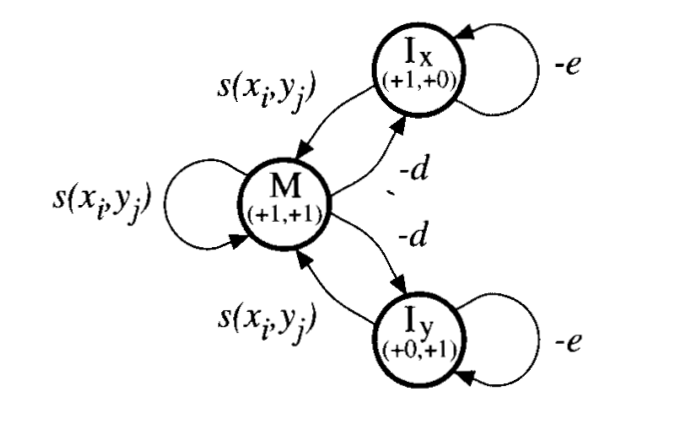
\includegraphics[width=0.5\linewidth]{automaton.png}}
	\caption{Diagram showing the three states.}
	\label{fig:automatom}
\end{figure}

Since we are on a semi-global alignment, we consider the best score equals to ${\text{max}[\text{max}(k_{n,1},\dots,k_{n,j}),\text{max}(k_{1,m},\dots ,k_{i,m})]}$ and we make the traceback from this point. In order to do it we need to consider, like in the problems above, which option was used to get the maximum value but this implies changing between states. Keeping in the state $I_x$ or $I_y$ means increasing the gap, and the state $M$ means a match.
\end{sloppypar}
\end{exercise}

\begin{exercise} % Task 6
For the local alignment with affine gaps, we can use an algorithm based in the Smith-Waterman algorithm, described in \cite{durbin}. It is a particular case where we consider, in addition to the possibilities of adding a gap to one or the other sequence or not adding a gap, the possibility of stopping or starting at that point. This is implemented as a change in the DP, by adding the case $0$ when getting the maximum score in the recursion. In other words, it is better to align the sequences locally than going with a negative score. This is done by changing the case in \thref{task:5} to ${k_{i,j}=\text{max}[k_{i-1,j}+Sc(s_i,t_j), p_{i,j}, q_{i,j},0]}$.
\end{exercise}

\begin{exercise} % Task 7
The algorithms presented so far are all exact, in a sense that they will return for sure the alignment with the best score but they all come with complexity of $\O(mn)$. If we use this to align a given sequence of size one thousand to a database of hundreds of millions of residues, the number of matrix entries will be the order of $10^{11}$ which would take a long time to compute, as explained in \cite{durbin}. We should keep in mind that the human genome, for example, has $3,0.10^9$ base pairs. In order to solve this problem, we can use heuristic algorithms that not necessarily return the best alignment but that can run much faster. Such a example is BLAST.

In order to do this task we will use the Aho-Corasick algorithm as described in \cite{pekka}. We start by creating the set $\W_g$ and from this set we create $\S_g$ by doing for each word of $\W_g$ the following procedure: we modify the first entry of this word by all the possibilities, meaning the entries of Blosum50, and we store those whose alignment score with the original sequence is greater than the defined threshold. 
\end{exercise}

\begin{exercise} % Task 8
	content...
\end{exercise}

\begin{commental}
For \thref{task:4} and \thref{task:5} we used MATLAB and Bioinformatics Toolbox Release 2016a in order to test our algorithm. This toolbox has an implementation of the cases we were handling, making us able to validate our code and fine minor errors in the implementation.
\end{commental}

\begin{commental} \thlabel{cmt:2}
We should keep in mind that as the diagram in figure \ref{fig:automatom} was extracted from \cite{durbin}, it does not use the same notation as us. The only purpose of this figure is to illustrate the three possibles states in the processes of finding the alignment.
\end{commental}

\begin{thebibliography}{3}
	
	\bibitem{jones} 
	Neil C. Jones and Pavel a. Pevzner. 
	\textit{an Introduction to Bioinformatics algorithms}. 
	MIT Press, 2004
	
	\bibitem{durbin} 
	Richard Durbin, Sean R. Eddy, anders Krogh and Graeme Mitchison. 
	\textit{Biological Sequence analysis: Probabilistic Models of Proteins and Nucleic acids}. 
	Cambridge University Press, 1998
	
	\bibitem{carl} 
	 Carl Kingsford. 
	\textit{Lecture Slides}. 
	 Available at \\ http://www3.cs.stonybrook.edu/~rp/class/549f14/lectures/CSE549-Lec04.pdf.
	
	\bibitem{pekka} 
	Pekka Kilpelainen. 
	\textit{Lecture Slides}. 
	Available at\\ https://www.cs.uku.fi/~kilpelai/BSA05/lectures/slides04.pdf
\end{thebibliography}

\end{document}
